% FIXME: rivedere se per ogni modello...
Per ogni modello, la creazione di training e validation set è stata realizzata 
utilizzando due tecniche diverse: è stato effettuato un esperimento in cui 
viene utilizzato un \textit{holdout} 80--20 ed uno che ricorre ad una 
\textit{10-fold cross validation}.

Per quanto riguarda l'holdout, vengono di seguito mostrate le distribuzioni dei 
dati nei due set:



\section{Random Forest}
Per l'addestrare è stato utilizzato il package R \texttt{RandomForest}.

\subsection{Holdout}
Nel primo esperimento, per creare training e validation set è stato utilizzato 
un \textit{holdout} 80--20.


La stima degli errori di classificazione OOB è stata di è del 7,06\%.\\

Le misure di accuracy, precision, recall e f-measure sono le seguenti:
\begin{figure}[H]
	\centering
	\begin{tabular}{lcccc}
		\toprule
		& \textbf{Accuracy} & \textbf{Precision} & \textbf{Recall} & 
		\textbf{F-Measure}  \\
		\midrule
		Training	& 94,41\% & 87,63\% & 38,65\% & 53,64\%    	\\ 
		Validation	& 93,11\% & 70,41\% & 28,33\% & 40,41\%   	\\ 
		\bottomrule
	\end{tabular}
	\captionof{table}{Analisi performance \textsc{Random Forest}}
	\label{tab:rf_performance}
\end{figure}

Di seguito vengono mostrate le curve ROC per il traning e il validation set:

\begin{figure}[htb]
	\centering
	\begin{subfigure}[t]{1\textwidth}
		\begin{minipage}[t]{0.475\textwidth}
			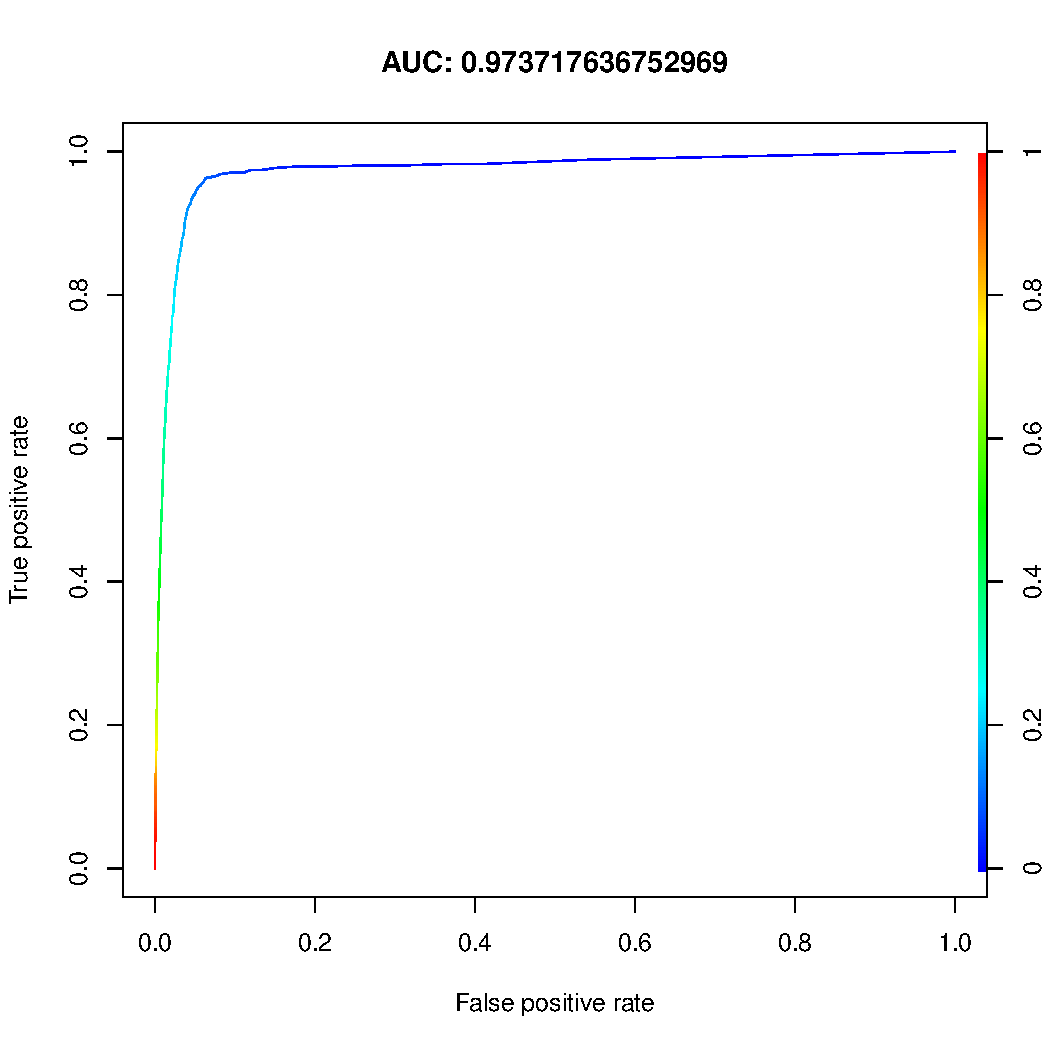
\includegraphics[width=\textwidth]{images/ml/random_forest/HoldoutRF/auc_train}
		\end{minipage}
		\hfill
		\begin{minipage}[t]{0.475\textwidth}
			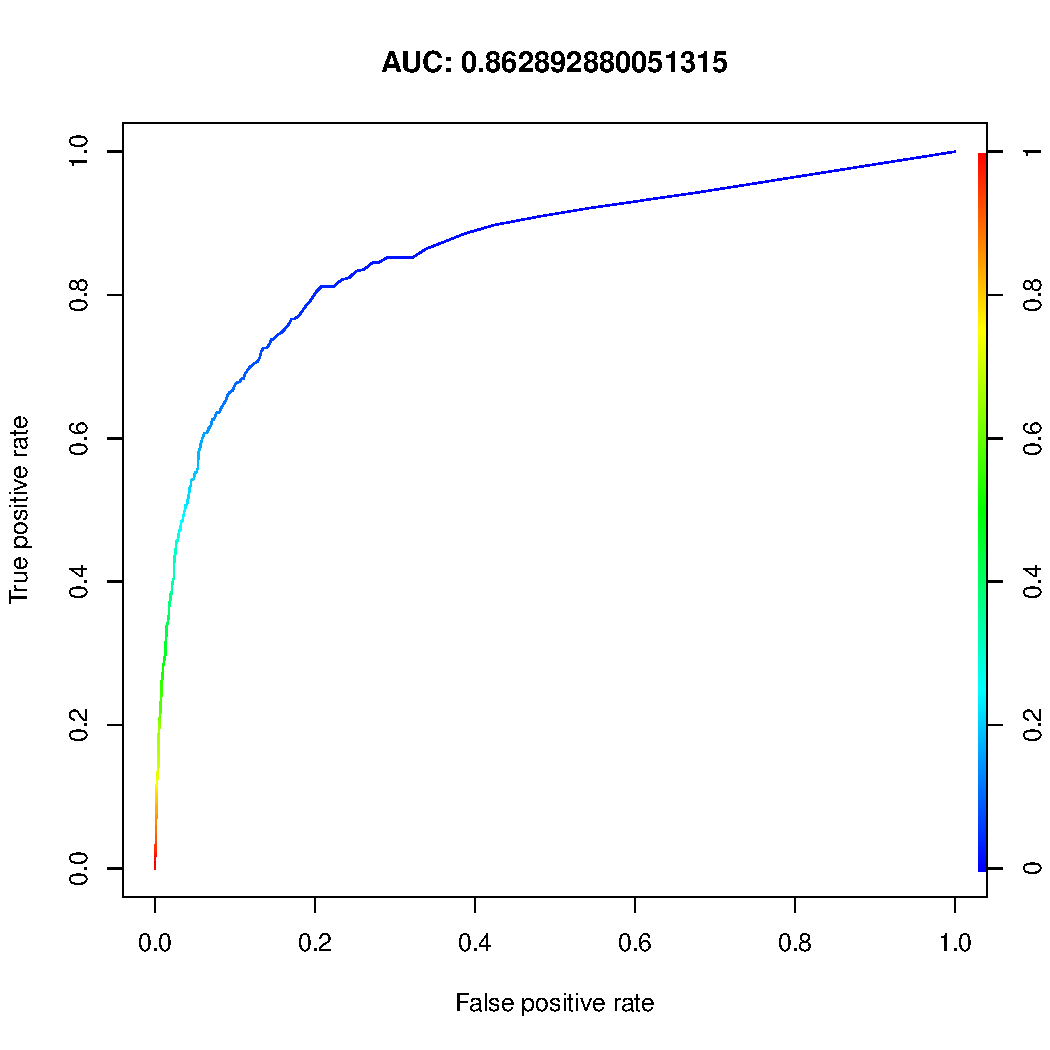
\includegraphics[width=\textwidth]{images/ml/random_forest/HoldoutRF/auc_test}
		\end{minipage}
	\end{subfigure}
	\caption{ROC sul training e validation set}
	\label{fig:rf_roc}
\end{figure}


\subsection{10-fold cross validation}
L’operazione di cross validation è stata eseguita sul modello basato su SVM 
dividendo il dataset in proporzione 90-10. Le performance ottenute sono 
superiori a quelle di par- tenza, abbiamo un’accuratezza complessiva dell’ 
84.08%, in tabella 3.1 sono mostrate le “matrici di confusione” relative ad 
%ogni fold.


% inserire matrice di confuzione cross validation (ogni fold)

% misure finali calcolate come la media delle misure su ogni fold (sia classe 
%positiva sia classe negativa)
%precision, recall, fmeasure 
%curde AUC er ogni fold sul validation

\subsubsection{Stima delle misure di performance}

\subsubsection{precision, recall, f-measure, area under curve per singola 
	classe e 
	complessiva}
